\documentclass{IOS-Book-Article}

\usepackage{xcolor}

%mystuff
\def\VIKTOR#1{\medskip\par\noindent\textcolor{blue}{\bf VIKTOR: #1}\par\medskip}
\def\KIRIL#1{\medskip\par\noindent\textcolor{red}{\bf KIRIL: #1}\par\medskip}

\usepackage{url}
\usepackage{graphicx}

\usepackage{mathptmx}



%\usepackage{times}
%\normalfont
%\usepackage[T1]{fontenc}
%\usepackage[mtplusscr,mtbold]{mathtime}
%
\def\hb{\hbox to 10.7 cm{}}

\begin{document}

%\pagestyle{headings}
\def\thepage{}

\begin{frontmatter}              % The preamble begins here.


%\pretitle{Pretitle}
\title{Converting Academic Papers in Biodiversity Science into Computer Knowledge\\\textbf{ {\normalsize Extended Abstract}}}

%\markboth{}{July 2017\hb}
%\subtitle{Subtitle}

\author[A,B]{\fnms{Senderov} \snm{Viktor}%
\thanks{Corresponding Author: Viktor Senderov, Pensoft Publishers, Prof. Georgi Zlatarski 12, 1700 Sofia, Bulgaria, E-mail: vsenderov@gmail.com.}},
\author[B]{\fnms{Simov} \snm{Kiril}}
and 
\author[A,B]{\fnms{Penev} \snm{Lyubomir}} 

\runningauthor{Senderov et al.}
\address[A]{Pensoft Publishers, Sofia, Bulgaria}
\address[B]{Bulgarian Academy of Sciences, Sofia, Bulgaria}

\begin{abstract}
A motivation and conceptual model of the OpenBiodiv ontology are presented. The ontology models the process by which biodiversity knowledge is described in scholarly publications. These publications are then converted to a knowledge graph about the diversity of life on Earth (The {Open} {Biodiversity} {Knowledge} {Management} {System}). Motivation, related works, main classes and properties, and a short discussion are presented in this extended abstract.
\end{abstract}

\begin{keyword}
ontology, biodiversity, knowledge graph, OWL, RDF, concept taxonomy
\end{keyword}
\end{frontmatter}
\markboth{July 2017\hb}{July 2017\hb}
%\thispagestyle{empty}
%\pagestyle{empty}

\section{Introduction}

In this work we present the motivation and the main conceptual model of the OpenBiodiv ontology---an ontology for The {Open} {Biodiversity} {Knowledge} {Management} {System}. We describe the domain of biodiversity publishing and more precisely we describe the modeling of taxonomic publications. We begin by presenting motivation and related works. Then we present the main classes and properties of the OpenBiodiv ontology.

Semantic publishing is bringing about a revolution in the field of biological science. In the biomedical domain there are well-established efforts to extract information and discover knowledge from literature \cite{r1, r2, r3}. The biodiversity domain, and in particular biological systematics (from here on in this paper referred to as \emph{taxonomy}), is also going in the direction of semantization of its research outputs \cite{r4,r5,r6}. In this contribution, we present our work to fill the missing gaps in ontology development in taxonomy, and to create a knowledge system based on taxonomic literature.

Taxonomy is a very old discipline dating back to possibly Aristotle, whose fundamental insight was to group living things in a hierarchy \cite{r7}. The discipline took its modern from after Carl Linnaeus (1707 - 1778) \cite{r7}. In his system, Linnaeaus proposed to group organisms into \emph{kingdoms, classes, orders, genera, and species}, give them scientific names consisting of Latinized bionomials, list possible alternative names, and give a characteristic description of the groups \cite{r8}. These groups are called taxa and give the name of the discipline.

Even though Linnaeus and his colleagues may have hoped to describe life on Earth during their lifetimes, we now know that there are millions of species still undiscovered and undescribed \cite{r9}. Moreover, with the advent of evolutionary biology, the grouping principles have changed \cite{r10}. Therefore, the description of life on Earth is a perpetual process and cannot be completed with a single project that can then be converted into an ontology. Thus, our aim is to create an ontology not of biodiversity itself, but to create a more generic ontology of the taxonomic process. The ongoing use of this ontology will enable the formal description of the totality of biodiversity knowledge at any given point in time.

Taxonomy works by employing the scientific method. Researchers examine specimens and based on the phenotypic and genetic variation that they observe form a hypothesis \cite{r11}. This hypothesis is called a taxon concept, a potential taxon, or---in the case of species-level taxa---a species hypothesis \cite{r12}. A taxon concept describes the allowable phenotypic and genomic variation within a taxon by both listing which specimens belong to it and by defining its characters explicitly. It is a valid falsifiable scientific claim as it needs to fulfill certain verifiable evolutionary requirements. For example, a species level concept needs fit our current understanding of what a species is, and a concept at a higher taxonomic level needs to form a monophyletic group \cite{r10}. Taxon concepts are published in the treatment section \cite{r13} of a scholarly taxonomic paper. Our ontology models scholarly taxonomic papers, taxon concepts, Latinized names, and other entities important in the taxonomic process.

The publishing domain has been modeled through the Semantic Publishing and Referencing Ontologies (SPAR) \cite{r14}. Taxonomic articles in particular have been modeled through the TaxPub XML schema \cite{r13}. Our bibliographic model has SPAR at its core with a few extensions that we've written to accommodate for TaxPub elements.

Occurrences of living things and sampling for specimens have previously been modeled through DarwinCore (DwC) and Darwin-Semantic Web (Darwin-SW) \cite{r15, r16}. We incorporate the Darwin-SW model in our ontology as it is.

Latinized names have previously been modeled through the NOMEN ontology\footnote{\url{https://github.com/SpeciesFileGroup/nomen}} and partly through the Taxonomic Nomenclatural Status Terms (TNSS) \cite{r17}. Latinized names are governed by the International Code of Zoological Nomenclature (ICZN) \cite{r18} and by the International Code of Nomenclature for algae, fungi, and plants (Melbourne Code) \cite{r19}. While NOMEN and the TNSS take a top-down approach of modeling the Codes, we take a bottom-up approach of modeling the actual usage of taxonomic names in articles. Where possible we map the classes that we've defined to NOMEN.

Taxon concepts have been modeled in XML through the Biodiversity Information Standards (TDWG) Taxonomic Concept Transfer Schema (TCS)\footnote{\url{http://www.tdwg.org/standards/117}}. A now defunct and unavailable taxon concept ontology had been previously developed\footnote{Taxon {Concept} {Ontology} developed by Peter DeVries. \url{http://taxonconcept.org}}. As we wanted to incorporate all of the semantic features of taxon concepts as discussed in the concept taxonomy literature \cite{r12, r20, r21}, we've modeled taxon concepts in OWL de novo.


\section{OpenBiodiv Ontology}

The OWL implementation of the OpenBiodiv ontology resides within a literate programming document\footnote{The {Open} {Biodiversity} {Knowledge} {Management} {System} {RDF} {Guide} developed by Viktor Senderov, Daniel Mietchen and Kiril Simov. \url{https://github.com/pensoft/OpenBiodiv/blob/master/ontology/RDF\_Guide.md}}. A key innovation of the ontology is that it introduces the class Taxonomic Name Usage (TNU)\footnote{The term TNU has been discussed previously widely in the community and we do not claim credit for coining it.} to connect bibliographic elements such as sections of the article, captions in a figure, etc. to biological names (Fig. \ref{TNU}). An example TNU would be "\emph{Heser stoevi} Deltschev, sp. n.". The cursive text is the Latinized bionomial name of the species, followed by an author, and the by a taxonomic status. The status indicates the sense it which the scientific name has been invoked (here "species novum" indicating a taxon discovery). The nomenclature of Latinized scientific names is highly complex, as governed by the Codes (synomies, replacement names due to homonymies, corrections of spelling mistakes, etc. \cite{r22}). Instead of modeling the Codes top-down, we've investigated the actual use of these statuses in around 4,000 articles published across four taxonomic journals (ZooKeys, Biodiversity Data Journal, PhytoKeys, and MycoKeys) to create a taxonomic status vocabulary\footnote{\url{https://github.com/pensoft/OpenBiodiv/blob/master/ontology/RDF\_Guide.md\#vocabulary-of-taxonomic-statuses}}.

Based on this vocabulary, with the help of several SPARQL rules\footnote{\url{https://github.com/pensoft/OpenBiodiv/blob/master/ontology/RDF\_Guide.md\#biological-names}}, it is possible to infer the validity of Latinized scientific names and to build chains of replacement names ("replacement name" is a transitive relation). The sink of the sub-graph formed in this way is always the current valid name for a taxon (Fig. \ref{name}). The relatedness of names can be also inferred on the basis of the co-occurrence of names in a specific part of the manuscript (nomenclature section). Another approach to infer related names, to which our approach will be compared, is the use of distributional semantics.

\begin{figure}[h!]
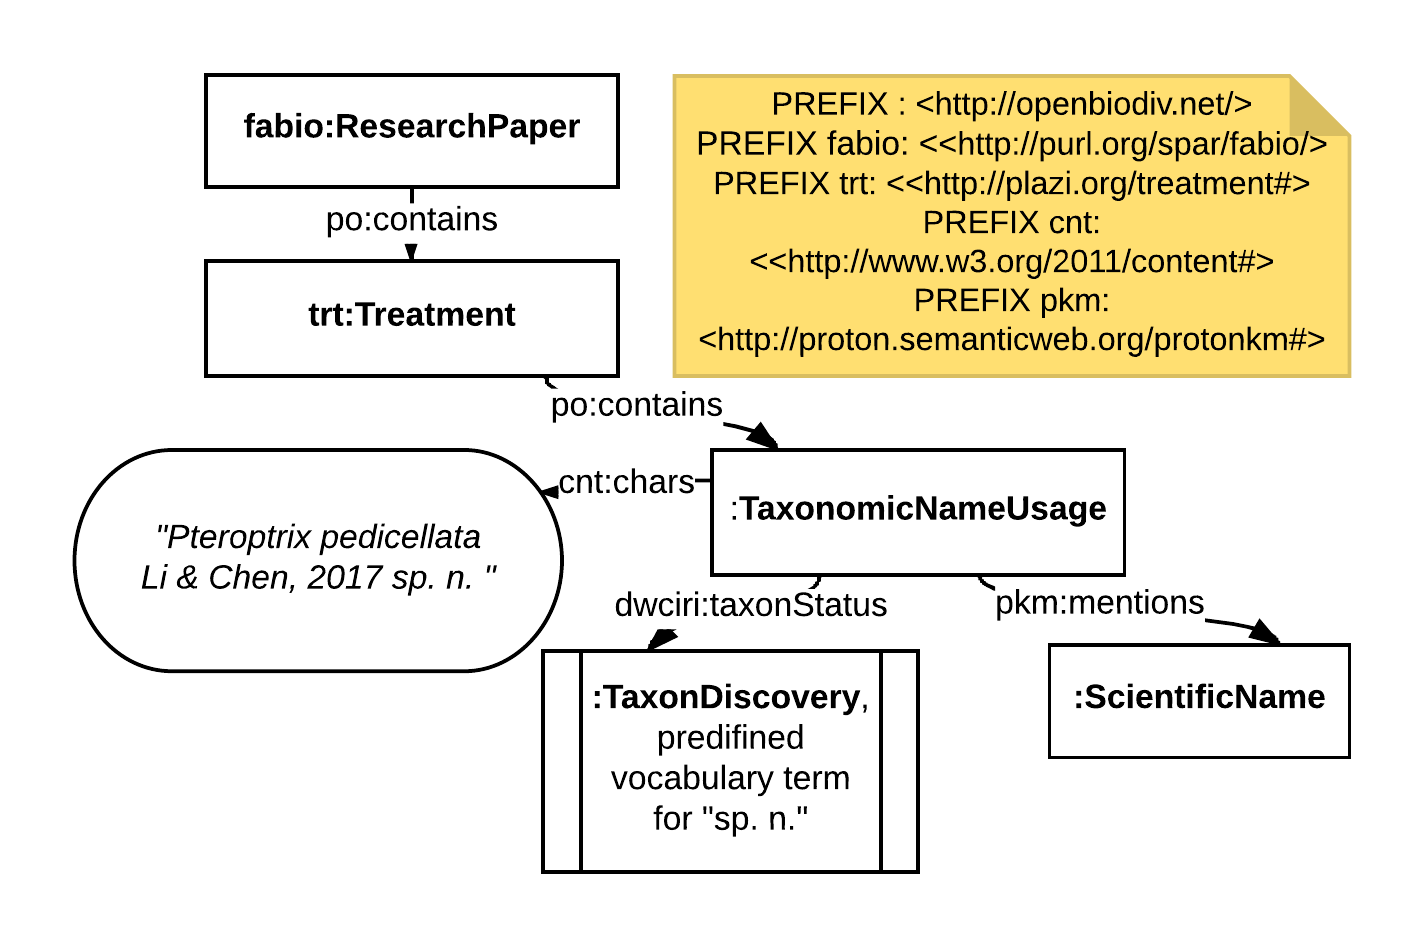
\includegraphics[width=\textwidth]{Extended_Abstract_Fig__1.png}
\caption{Taxonomic Name Usage is class that connects document elements (parts of the paper) to biological names (e.g. scientific names). The context is carried by a taxonomic status.}
\label{TNU}
\end{figure}

\begin{figure}[h!]
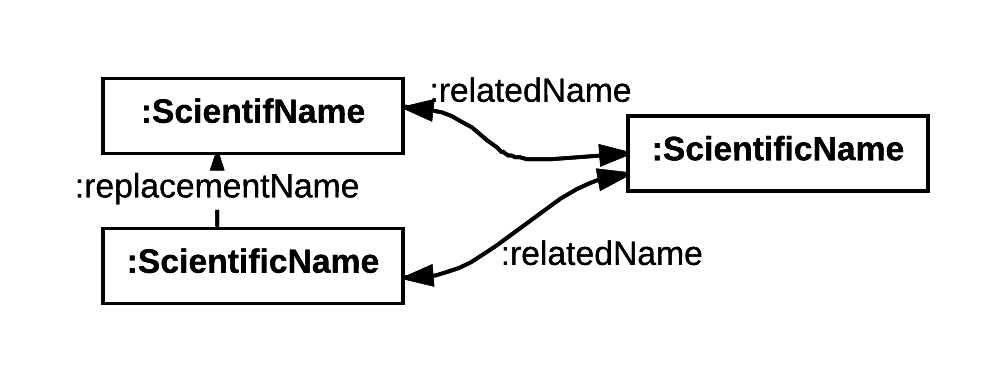
\includegraphics[width=\textwidth]{Extended_Abstract_Fig_2.png}
\caption{Chains of replacement names can be followed to find the currently valid name. {\tt :relatedName} indicates that two names are related somehow, but not which is preferable.}
\label{name}
\end{figure}

It is important to note, however, that in our ontology names are not the carriers of the semantic information about a taxon. This task is accomplished by the class Taxon Concept. It is intensionally equivalent to DarwinCore's Taxon\footnote{\url{http://rs.tdwg.org/dwc/terms/\#Taxon}}. However, by including "concept" in the class' name, we hightlight the fact that the  semantics it carries reflect the scientific theory of a given author about a taxon in nature. Thus, our ontology allows for multiplicity of opinion: a given scientific name may be linked to different taxon concepts (reflecting for example the gradual accumulation of knowledge about the taxon over time, or perhaps even concurrent disagreement between authors). Last, we modeled not only simple parent-child relationship between taxon concepts, but also relationships of partial overlap, disjointness, equality, proper inclusion, and inverse proper inclusion, both intensively and intensionally as defined by the Region Connection Calculus-5\footnote{\url{https://en.wikipedia.org/wiki/Region\_connection\_calculus}}.

Our ontology serves as the basis for the Open Biodiversity Knowledge Management System (OBKMS, or OpenBiodiv) \cite{r5}. Currently, the system is under development with millions of triples and thousands of articles already having been processed. The usefulness of the ontology will be determined by how well it serves the needs of OpenBiodiv. One of its strong-points is that by filling the ontological gaps it allows the creation of a biodiversity knowledge graph \cite{r23}, and linking all taxonomic information together: occurrences, specimens, names, taxon concepts, articles, treatments, images, etc. This will allow the users of the system to answer competency questions\footnote{\url{http://wiki.pro-ibiosphere.eu/wiki/Competency\_Questions\_for\_RDF\_Treatments}}.

%\bibliographystyle{bmc-mathphys} % Style BST file (bmc-mathphys, vancouver, spbasic).
%\bibliography{bmc_article}

\begin{thebibliography}{99}

\bibitem{r1}
Momtchev, Vassil, Peychev, Deyan, Primov, Todor and Georgiev, Georgi. Expanding the pathway and interaction knowledge in linked life data. In: \textit{Proc. of International Semantic Web Challenge}, 2009, 

\bibitem{r2}
Williams, Antony J., Harland, Lee, Groth, Paul, Pettifer, Stephen, Chichester, Christine, Willighagen, Egon L., Evelo, Chris T., Blomberg, Niklas, Ecker, Gerhard, Goble, Carole, Mons, Barend, Open {PHACTS}: semantic interoperability for drug discovery, 
\textit{Drug Discovery Today} \textbf{17}, \textbf{21--22}, (2012), 1188--1198.

\bibitem{r3}
Rebholz-Schuhmann, Dietrich, Kirsch, Harald, Couto, Francisco. Facts from text—is text mining ready to deliver? \textit{PLoS biology}, \textbf{17}, \textbf{21--22}, (2005).

\bibitem{r4}
Tzitzikas, Yannis, Allocca, Carlo, Bekiari, Chryssoula, Marketakis, Yannis, Fafalios, Pavlos, Doerr, Martin, Minadakis, Nikos, Patkos, Theodore, Candela, Leonardo. Integrating heterogeneous and distributed information about marine species through a top level ontology. \textit{Research {Conference} on {Metadata} and {Semantic} {Research}}, (2013), pp. 289--301.

\bibitem{r5}
Senderov, Viktor and Penev, Lyubomir. The {Open} {Biodiversity} {Knowledge} {Management} {System} in {Scholarly} {Publishing}. \textit{Research Ideas and Outcomes}, \textbf{2}, (2016).

\bibitem{r6}
Renner, Susanne. Fast, linked, and open – the future of taxonomic publishing for plants: launching the journal {PhytoKeys}. \textit{PhytoKeyss}, \textbf{1}, (2010).

\bibitem{r7}
Manktelow, Mariette. History of taxonomy. \textit{Lecture from Dept. of Systematic Biology, Uppsala University}, (2010), http://www.atbi.eu/summerschool/files/summerschool/Manktelow\_Syllabus.pdf.

\bibitem{r8}
Linnaeus, Carl von, and Salvius, Lars. Caroli Linnaei...Systema naturae per regna tria naturae :secundum classes, ordines, genera, species, cum characteribus, differentiis, synonymis, locis. V 1. \textit{Holmiae :Impensis Direct. Laurentii Salvii}, (1758), pages 881.

\bibitem{r9}
Ratnasingham, Sujeevan and Hebert, Paul D. N. A {DNA}-{Based} {Registry} for {All} {Animal} {Species}: {The} {Barcode} {Index} {Number} ({BIN}) {System}. \textit{PLoS ONE}, \textbf{8, 7}, (2013).

\bibitem{r10}
Mallet, James. Species, concepts of. \textit{Encyclopedia of biodiversity},\textbf{5}, (2001), pp. 427--440.

\bibitem{r11}
Deans, Andrew R., Yoder, Matthew J., Balhoff, James P. Time to change how we describe biodiversity. \textit{Trends in Ecology \& Evolution}, \textbf{27, 2}, (2012), pp. 78--84.

\bibitem{r12}
Berendsohn, Walter G. The concept of" potential taxa" in databases. \textit{Taxon}, (1995), pp. 207--212.

\bibitem{r13}
Catapano, Terence. {TaxPub}: an extension of the {NLM}/{NCBI} journal publishing {DTD} for taxonomic descriptions. (2010).


\bibitem{r14}
Peroni, Silvio. The semantic publishing and referencing ontologies. \textit{Semantic {Web} {Technologies} and {Legal} {Scholarly} {Publishing}}. Springer. (2014), pp. 121--193.

\bibitem{r15}
Baskauf, Steve, Webb, Campbell O. Darwin-{SW}: {Darwin} {Core}-based terms for expressing biodiversity data as {RDF}. \textit{Semantic Web Journal}, \textbf{7, 6}, (2016), pp. 629--643.

\bibitem{r16}
Wieczorek, John, Bloom, David, Guralnick, Robert, Blum, Stan, Döring, Markus, Giovanni, Renato, Robertson, Tim, Vieglais, David. Darwin {Core}: {An} {Evolving} {Community}-{Developed} {Biodiversity} {Data} {Standard}. \textit{PLoS ONE}, \textbf{7, 1}, (2012).

\bibitem{r17}
Morris, Paul J. and Morris, Robert A. and Wang, Zhimin. Taxonomic {Nomenclatural} {Status} {Terms}.

\bibitem{r18}
{The International Trust for Zoological Nomenclature, London, UK}. International {Code} of {Zoological} {Nomenclature}. (1999)

\bibitem{r19}
McNeill, John and International Association for Plant Taxonomy (eds.). International code of nomenclature for algae, fungi and plants ({Melbourne} code): adopted by the {Eighteenth} {International} {Botanical} {Congress} {Melbourne}, {Australia}, {July} 2011. (2012).

\bibitem{r20}
Franz, N.M. and Peet, R.K. Perspectives: {Towards} a language for mapping relationships among taxonomic concepts. \textit{Systematics and Biodiversity}, \textbf{V. 7, 1}, (2009), pp. 5--20.

\bibitem{r21}
Sterner, Beckett and Franz, Nico M. Taxonomy for {Humans} or {Computers}? {Cognitive} {Pragmatics} for {Big} {Data}. \textit{Biological Theory}, \textbf{V. 12, 2}, (2017), pp. 99--111.

\bibitem{r22}
Patterson, David, Dmitry Mozzherin, David Shorthouse, and Anne Thessen. “Challenges with Using Names to Link Digital Biodiversity Information.” Biodiversity Data Journal 4 (May 25, 2016): e8080. doi:10.3897/BDJ.4.e8080.

\bibitem{r23}
Page, Roderic. “Towards a Biodiversity Knowledge Graph.” Research Ideas and Outcomes 2 (April 7, 2016): e8767. doi:10.3897/rio.2.e8767.


\end{thebibliography}


\end{document}
